\section{$B^+$-Tree}

\begin{frame}
\frametitle{$B^+$-Tree}

\textbf{Advantages}
\begin{itemize}
\item Optimized for CPU cache performance
\item Prefered index struture for memory-resident data
\end{itemize}

\textbf{Problems on PCM}
\begin{itemize}
\item Incurs a lot of writes on update/delete
\end{itemize}
\end{frame}

\begin{frame}
\frametitle{Algorithmic Challenges \& Goals}
\textbf{Challenges}
\begin{itemize}
\item High energy consumption (on write)
\item High latency \& low bandwith (on write)
\item Limited endurance
\end{itemize}

\textbf{Goals}
\begin{itemize}
\item Low computational complexity
\item Good CPU cache performance
\item Power efficiency
\end{itemize}
\end{frame}


\begin{frame}
\frametitle{SS}

\begin{itemize}
\item .
\end{itemize}

\end{frame}




\subsection{Variants}

\begin{frame}
\frametitle{$B^+$-Tree Node Variantes}
\begin{tabular}[t]{l r}
Ordered  & \\
& 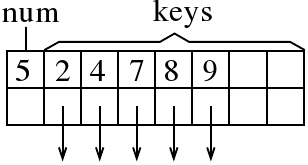
\includegraphics[scale=0.25]{images/ordered.png} \\
Unordered & \\
& 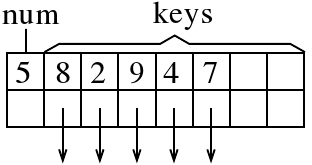
\includegraphics[scale=0.25]{images/unordered.png} \\
Bitmap & \\
&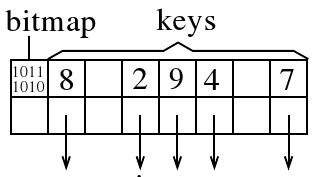
\includegraphics[scale=0.25]{images/bitmap.png}
\end{tabular}


\end{frame}



\subsection{$B^+$-Tree Variants}
\begin{frame}
\frametitle{Variants}

\begin{itemize}
\item Sorted
\item Unsorted
\item Unsorted Leaf
\item Unsored Leaf with bitmap
\end{itemize}

\end{frame}